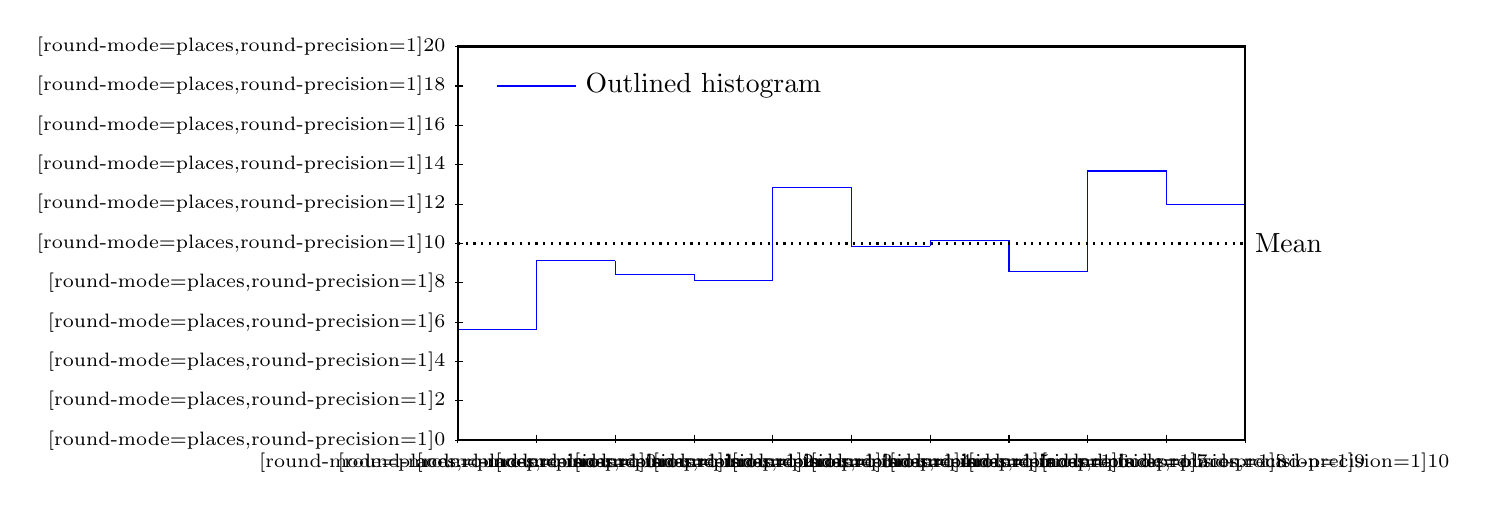
\begin{tikzpicture}
\begin{scope}
\clip (0,0) rectangle (10,5);
\draw[blue] (0.0,1.4091642297516938) -- (1.0,1.4091642297516938);
\draw[blue] (1.0,1.4091642297516938) -- (1.0,2.2802300388334156) -- (2.0,2.2802300388334156);
\draw[blue] (2.0,2.2802300388334156) -- (2.0,2.105932955534761) -- (3.0,2.105932955534761);
\draw[blue] (3.0,2.105932955534761) -- (3.0,2.027388033545427) -- (4.0,2.027388033545427);
\draw[blue] (4.0,2.027388033545427) -- (4.0,3.211134486407473) -- (5.0,3.211134486407473);
\draw[blue] (5.0,3.211134486407473) -- (5.0,2.4656617039649023) -- (6.0,2.4656617039649023);
\draw[blue] (6.0,2.4656617039649023) -- (6.0,2.538701869600402) -- (7.0,2.538701869600402);
\draw[blue] (7.0,2.538701869600402) -- (7.0,2.143674847456264) -- (8.0,2.143674847456264);
\draw[blue] (8.0,2.143674847456264) -- (8.0,3.41996593799481) -- (9.0,3.41996593799481);
\draw[blue] (9.0,3.41996593799481) -- (9.0,2.995646505175429) -- (10.0,2.995646505175429);
\end{scope}
\draw (0,2pt) -- (0, -1pt) node[below] {\scriptsize{\num[round-mode=places,round-precision=1]{0}}};
\draw (1,2pt) -- (1, -1pt) node[below] {\scriptsize{\num[round-mode=places,round-precision=1]{1}}};
\draw (2,2pt) -- (2, -1pt) node[below] {\scriptsize{\num[round-mode=places,round-precision=1]{2}}};
\draw (3,2pt) -- (3, -1pt) node[below] {\scriptsize{\num[round-mode=places,round-precision=1]{3}}};
\draw (4,2pt) -- (4, -1pt) node[below] {\scriptsize{\num[round-mode=places,round-precision=1]{4}}};
\draw (5,2pt) -- (5, -1pt) node[below] {\scriptsize{\num[round-mode=places,round-precision=1]{5}}};
\draw (6,2pt) -- (6, -1pt) node[below] {\scriptsize{\num[round-mode=places,round-precision=1]{6}}};
\draw (7,2pt) -- (7, -1pt) node[below] {\scriptsize{\num[round-mode=places,round-precision=1]{7}}};
\draw (8,2pt) -- (8, -1pt) node[below] {\scriptsize{\num[round-mode=places,round-precision=1]{8}}};
\draw (9,2pt) -- (9, -1pt) node[below] {\scriptsize{\num[round-mode=places,round-precision=1]{9}}};
\draw (10,2pt) -- (10, -1pt) node[below] {\scriptsize{\num[round-mode=places,round-precision=1]{10}}};
\draw (2pt,0.    ) -- (-1pt,0.    ) node[left] {\scriptsize{\num[round-mode=places,round-precision=1]{0}}};
\draw (2pt,0.5    ) -- (-1pt,0.5    ) node[left] {\scriptsize{\num[round-mode=places,round-precision=1]{2}}};
\draw (2pt,1.    ) -- (-1pt,1.    ) node[left] {\scriptsize{\num[round-mode=places,round-precision=1]{4}}};
\draw (2pt,1.5    ) -- (-1pt,1.5    ) node[left] {\scriptsize{\num[round-mode=places,round-precision=1]{6}}};
\draw (2pt,2.    ) -- (-1pt,2.    ) node[left] {\scriptsize{\num[round-mode=places,round-precision=1]{8}}};
\draw (2pt,2.5    ) -- (-1pt,2.5    ) node[left] {\scriptsize{\num[round-mode=places,round-precision=1]{10}}};
\draw (2pt,3.    ) -- (-1pt,3.    ) node[left] {\scriptsize{\num[round-mode=places,round-precision=1]{12}}};
\draw (2pt,3.5    ) -- (-1pt,3.5    ) node[left] {\scriptsize{\num[round-mode=places,round-precision=1]{14}}};
\draw (2pt,4.    ) -- (-1pt,4.    ) node[left] {\scriptsize{\num[round-mode=places,round-precision=1]{16}}};
\draw (2pt,4.5    ) -- (-1pt,4.5    ) node[left] {\scriptsize{\num[round-mode=places,round-precision=1]{18}}};
\draw (2pt,5.    ) -- (-1pt,5.    ) node[left] {\scriptsize{\num[round-mode=places,round-precision=1]{20}}};
\draw[thick] (0,0) rectangle (10,5);
\draw[thick,dotted] (0.0,2.5) -- (10.0,2.5);
\node[right] at (10.0,2.5) {Mean};
\draw[blue] (0.5,4.5) -- (1.5,4.5);
\node[right,] at (1.5,4.5) {Outlined histogram};
\end{tikzpicture}
%%% Local Variables: 
%%% mode: latex 
%%% TeX-master: "master" 
%%% End:

